\subsection{DQN in customized environments}

In this third section of the first part, we present frameworQ, a python framework for applying deep Q-learning algorithms in customized environments, developed during the first half of the internship. DQN algorithms are notoriously difficult to implement and debug, and reproducibility is a major issue in the field of deep reinforcement learning. With frameworQ, we aim at providing a ready-to-use and flexible baseline of DQN algorithms and environment wrappers to facilitate research, allowing to generate results faster by putting the focus on designing environments and their action/observation/reward functions, and hyper-parameter tuning. We first present the framework architecture and implementation, then describe global guidelines to tune hyper-parameters in practice, and finally demonstrate the proof of concept with two toy environments. The framework was used as a base code for the internship project in the second half of the internship. frameworQ is available at: \textbf{\url{https://github.com/romainducrocq/frameworQ}}.

\subsubsection{Presentation of frameworQ} \label{basics}

\textbf{Overview} \\
frameworQ is a python framework developed to facilitate research applications based on deep Q-learning algorithms. It provides a ready-to-use and fully abstracted DQN code baseline, and additional features and tools, in a standalone package, and entry scripts for training, testing, visualizing and comparing agents, with flexible command line control. It allows users to focus solely on creating customized environments, in an environment dedicated package, following a simple MVC prepared structure. As such, we intent to minimize the implementation effort and make deep Q-learning research more accessible. \\

\textbf{Global architecture} \\
frameworQ runs under a python virtual environment \texttt{venv/}, and an installation script is provided to build frameworQ and its dependencies, at \texttt{bin/make.sh}. The DQN code baseline is encapsulated in the \texttt{dqn/} package, and requires no modification, i.e. it is intended to be fully abstracted from the user. The customized environment is to be created in the \texttt{env/} package, and splitted into model, view and controller within structured templates, which consists of the only code to adapt. Three main scripts are used as entry points to the programs, \texttt{train.py} to train an agent with a set of hyper-parameters, \texttt{observe.py} to deploy a trained neural network for testing, and \texttt{play.py} to load the environment with non-DQN controllers for comparison. These can be launched from command lines with arguments or from shell scripts in \texttt{bin/}, as well as additional tools for visualizing learning curves and evaluation metrics. Two more folders \texttt{save/} and \texttt{logs/} respectively store trained models and log files, which are singled into \texttt{train/} and \texttt{test/}.

\pagebreak

\textbf{DQN baseline in \texttt{dqn/}} \\
The \texttt{dqn/} package groups the ready-to-use DQN baseline code, and implements the four algorithms presented in section 2; i.e. DQN, DDQN, 3DQN and Per3DQN; and further improvements presented hereafter, fully abstracted from the user. It is based on \texttt{Pytorch}, a heavily optimized machine learning library for tensor operations in neural networks, on both CPU and GPU. \texttt{agent.py} implements the agent, with the TD update for the four algorithms, the action-selection policy, the transition to tensor conversion and the training logs. These logs, i.e. the averaged rewards and durations over the last 100 episodes, are written to \texttt{.tfevents} log files in the \texttt{logs/train/} folder every $f_l$ timesteps, a log frequency defaulted to 1000 timesteps, with \texttt{Tensorboard}, a toolkit to visualize learning curves over training and evaluate agents. \texttt{network.py} implements the neural networks for online and target $Q$-networks, with both simple and dueling architectures, and dynamic model saving and loading. The model, i.e. the weights $\Theta_t(, \iota_t, \kappa_t)$ of the online $Q$-network $Q$ at timestep $t$, are saved to binary \texttt{.pack} files in the \texttt{save/} folder every $f_s$ timesteps, a save frequency defaulted to 10000 timesteps, with \texttt{msgpack}, an efficient object serialization library for \texttt{numpy} arrays. \texttt{replay\_memory.py} implements the replay memory data buffer, with both uniform and prioritized transition sampling. \texttt{env\_wrap.py} wraps the customized environment in \texttt{OpenAi Gym}, a reinforcement learning toolkit for simulated environments with many features, and writes the test logs, i.e. additional transition information defined by the user, as \texttt{.csv} files in the \texttt{/logs/test/} folder for further analysis. \texttt{env\_make.py} instantiates the customized environment and implements multi-processing training with \texttt{SubprocVecEnv}, a vectorization tool for training multiple environments in parallel over sub-processes. Finally, the \texttt{utils/} folder contains the implementation of the sum tree, a meta-class definition and all the dependencies of the aforementioned tools. 
\\

\textbf{Customized environment in \texttt{env/}} \\
The \texttt{env/} package contains a simple model, view, controller template structure for the creation of customized environments, and a hyper-parameter configuration file, and is the only code to be adapted in frameworQ. The model of the environment, i.e. all the object classes and additional resources, must be defined in the \texttt{custom\_env/} folder. The controller of the environment must be wrapped in \texttt{dqn\_env.py} in a DQN oriented structure, with action space size $|A|$ and state feature size $|s|$, observation pre-processing function $\phi$, reward function $R$, terminal state function, environment reset function and transition dynamics function $P$ for one timestep $t$, and optionally additional transition log information, and logic functions for the view only. A view can be optionally set for the environment in \texttt{view.py}, with either a template provided in \texttt{Pyglet}, a python interface for the graphics library \texttt{OpenGl}, or an empty wrapper for customized views. The view is activated only at deployment, and not during training for resource optimization, and can be disabled fully. The hyper-parameter configuration file \texttt{dqn\_config} contains all the hyper-parameters of the DQN algorithms to be tuned, as well as the neural network architecture, the loss function and the gradient optimizer. Default values for all those are provided as a starting point for tuning. A full guide for building customized environments can be found in \texttt{doc/}. \\

\textbf{Code modularity and flexible command control} \\
frameworQ is developed in a modular object-oriented paradigm, with extensive functional decomposition and class inheritance, in order to be easily maintained and updated. Moreover, it is designed such that DQN algorithms can be added towards full rainbow DQN. The main program scripts \texttt{train.py}, \texttt{observe.py} and \texttt{play.py} allow abundant line command control for flexible use, with the complete list of arguments detailed again in \texttt{doc/}.

\subsubsection{Further optimization, Per3DQN+} \label{basics}

\textbf{Optimized implementation} \\
Additionnaly to the four algorithms presented in section 2; i.e. DQN, DDQN, 3DQN and Per3DQN; frameworQ incorporates further optimization features that have been picked from the recent ML / RL literature, in an effort to maximize learning speed and stability:
\begin{itemize}
\setlength\itemsep{-0.5em}
  \item \textbf{MinMax scaling}: Neural networks are very sensitive to the range of input features, and  normalization in $[-1,1]$ both accelerates learning and reduces the risk for exploding gradients. In supervised learning, where the data distribution is known, it is common practice to normalize by Z-score. However, in reinforcement learning, as the data is online, we prefer to include min-max scaling in $[0, 1]$ in the observation pre-processing function $\phi$. If the bounds for input features are unknown, data are scaled by the minimum and maximum values encountered at that time of training:
  \[ MinMax(x) = \frac{x - x_{max}}{x_{min} - x_{max}}, Z-score(x) = \frac{x - \mu}{\sigma} \]
  \item \textbf{Exponential decay}: The explore-exploit trade-off has been empirically found to have a better balance with exponential decay, with $\epsilon$-decay slowing down over time:
  \[ 
  \text{Exponential decay: } \epsilon = 
  \begin{cases}
      \exp(t \cdot \frac{\log(\epsilon_{min})}{\epsilon_{dec}}) & \text{if } t < \epsilon_{dec}\\
      \epsilon_{min} > 0 & \text{else}
  \end{cases}
  \]
  \item \textbf{ELU activation}: ReLU non-linearities don't handle negative inputs and are subject to vanishing gradients, causing the dying ReLU problem. The exponential linear unit activation (ELU) is a similar identity function and a strong alternative to ReLU that can produce smooth small negative outputs in $[-1,0]$ for negative values:
  \[
  ELU(z)=
  \begin{cases}
      z & \text{if } z > 0 \\
      e^z - 1 & \text{else}
  \end{cases}
  \]
  \item \textbf{Huber loss}: Deep Q-learning is extremely sensitive to outliers in the training data, and the MSE loss, while efficient, introduces instability with the square term. The Huber loss provides a robust substitute, by alternating between the mean square error L2-loss for small values of the TD error magnitude and the mean absolute error L1-loss for larger values, a stabilization method called gradient error clipping:
  \[ 
  \text{Huber loss: } L_t(\delta_t, w_t) = \frac{1}{2M}\sum_{m=1}^M w_t^{(m)} \cdot
  \begin{cases}
      \text{MSE L2-Loss: }(\delta_t^{(m)})^2 & \text{if } |\delta_t^{(m)}| < 1 \\
      \text{MAE L1-Loss: }2 \cdot |\delta_t^{(m)}| - 1 & \text{else}
  \end{cases}
  \]
  \item \textbf{Adam optimizer}: Gradient descent faces limited performances in deep neural networks, due to slow convergence. The adaptive moment estimation optimizer (Adam) [9] (Kingma, Ba, 2017), speeds up parameter optimization by correcting the gradient update with a momentum correction term $v_t$ and a root mean square propagation term $s_t$ (RMSprop), with learning rate $\alpha$ and coefficients $\beta_1$, $\beta_2$ and $\epsilon$:
  \[ 
  \text{Adam optimizer: } 
  \begin{cases}
      v_t = \frac{\beta_1 \cdot v_{t-1} + (1 - \beta_1) \cdot \Delta_{i,j}^{(l)}}{1-\beta_1^t} & \text{with } v_0=0, \beta_1 = 0.9\\
      s_t = \frac{\beta_2 \cdot s_{t-1} + (1 - \beta_2) \cdot \Delta_{i,j}^{2(l)}}{1-\beta_2^t} & \text{with } s_0=0, \beta_2 = 0.999\\
      \Theta_{i,j}^{(l)} = \Theta_{i,j}^{(l)} - \alpha \cdot \frac{v_t}{\sqrt{s_t} + \epsilon} & \text{with } \epsilon = \num{1e-8}\\
  \end{cases}
  \]
  \item \textbf{Polyak update}: The target $\hat{Q}$-network $\hat{Q}$ is updated by hard copy of the $Q$-network $Q$ every $C$ steps, the target update frequency. This causes learning to be unstable for a small time interval after copies, when the correlation between TD targets and online Q-values is still strong, and makes the Q-function sometimes diverge locally. The Polyak soft update [10] (Lillicrap et al., 2019) smoothes the updates by updating the weights $\Theta_t^-$ of the target $\hat{Q}$-network $\hat{Q}$ by a very small rate $\tau$ of the weights $\Theta_t$ of the $Q$-network $Q$ at each time step $t$. Thus, $\hat{Q}$ always converges towards $Q$, but with a sufficient delay for decorrelation between TD targets and online Q-values:
  \[ \Theta^-_t = (1-\tau) \cdot \Theta^-_t + \tau \cdot \Theta_t \text{, with } \tau \ll 1\]
  \item \textbf{Action repeat}: The time steps $t$ do not have to coincide with the real clock rate of the environment $\varepsilon$. Moreover, knowing that difficulty of performing optimal sequences of actions rises with the horizon $T$, learning can strongly benefit from adjusting the action interval to an optimal decision frequency for the task. At each time step $t$, the action $a_t$ is repeated $k$ times in the environment $\varepsilon$, and the reward $r_{t+1}$ is obtained by accumulating the intermediate rewards, such that $r_{t+1} = \sum_k r_k$.
  \item \textbf{Time limit}: In early phases of learning, it often happens that the best known policy is simply to avoid terminal states, associated with penalties. The agent thus starves, and selects sub-optimal actions that, while performing poorly, extend the episode. A time limit is set on episodes to avoid cases of starving, i.e. early stopping.
\end{itemize}

\pagebreak

\textbf{Combining everything with Per3DQN+} \\
In frameworQ, by combining the four algorithms presented in section 2; i.e. vanilla, double, dueling and Per DQN; and the additional improvements presented hereinabove, we obtain the algorithm used for the internship project, presented later on in the second part. We call this algorithm the Per3DQN+ algorithm for simplicity, and it is as follows:

\begin{algorithm}[H]
\small
\caption*{Per3DQN+ algorithm}
\begin{algorithmic}
    \STATE Initialize step $t = 0$;
    \STATE Initialize the online dueling $Q$-network $Q$ with random weights $\vartheta_0 = (\Theta_0, \iota_0,\kappa_0)$;
    \STATE Initialize the target dueling $\hat{Q}$-network $\hat{Q}$ with weights $\vartheta^-_0 =  (\Theta^-_0, \iota^-_0,\kappa^-_0) = \vartheta_0$;
    \STATE Initialize the replay memory buffer $D$ to capacity $N$
    \STATE with $Nmin$ random transitions $(s,\text{rand }a \in A,s',r')$;
    \STATE Initialize the sum tree to capacity $2N - 1$ with zero-padding;
    \FOR{episode e = 1:E}
        \bindent
        \STATE Initialize sequence, observe initial state $s_t=\phi(x_t) \sim MinMax$;
        \WHILE{$s_t$ not terminal \textbf{and} time not limit}
            \bindent
            \STATE With probability $\epsilon$ select a random action $a_t \in A$
            \STATE otherwise select action $a_t = arg\max_{a}Q_{\pi,t}(s_t,a,\vartheta_t)$;
            \FOR{repeat k=1:K}
                \bindent
                Execute $a_t$ in emulator $\varepsilon$ and accumulate reward $\sum_k r_k$;
                \eindent
            \ENDFOR
            \STATE Observe reward $r_{t+1}$ and next state $s_{t+1}=\phi(x_{t+1}) \sim MinMax$;
            \STATE Store prioritized transition $(s_t,a_t,s_{t+1},r_{t+1}, p_{max})$
            \STATE with $(s_t,a_t,s_{t+1},r_{t+1})$ in $D$ and $p_{max}$ in the sum tree;
            \STATE Sample prioritized batch $P(D)$ of $M$ transitions $(s,a,s',r',p_i)^{(m)}$, with $P(i) = \frac{p_i}{\sum_j p_j}$
            \STATE with $p_i^{(m)}$ in the sum tree and $(s,a,s',r')^{(m)}$ in $D$, with the sum tree sample algorithm;
            \FOR{m = 1:M}
                \bindent
                \STATE Set double TD error $\delta^{(m)}_t = r'^{(m)} + \gamma \cdot Q_{\pi,t}(s'^{(m)},arg\max_{a'}Q_{\pi,t}(s'^{(m)},a',\vartheta_t),\vartheta^-_t)$ \\ \;\;\;\;\;\;\;\;\;\;\;\;\;\;\;\;\;\;\;\;\;\;\;\;\;\;\;\;\;\;\;\;\;\;\;\;\;\;\;\;\;\;\;
                $-$ $Q_{\pi,t}(s^{(m)},a^{(m)},\vartheta_t)$;
                \STATE Set priority $p_i^{(m)}= min(|\delta^{(m)}_t| + \xi, 1)^{\eta}$;
                \STATE Update priority $p_i^{(m)}$ in the sum tree, with the sum tree update algorithm;
                \STATE Set IS weight $w_{t}^{(m)} = (N_t \cdot P(i))^{-\beta} / \max w_{t} = (\frac{p_i^{(m)}}{p_{min}})^{-\beta}$;
                \eindent
            \ENDFOR
            \STATE Perform an Adam optimizer step on Huber loss $L_t(\delta_t,w_t)$ w.r.t. $\vartheta_t$, with $\Delta_t$, $\alpha$;
            \STATE Soft update target $\hat{Q}$-network $\hat{Q}$ with Polyak update, with $\vartheta^-_t = (1-\tau) \cdot \vartheta^-_t + \tau \cdot \vartheta_t$;
            \STATE Save model every $f_s$ steps, log metrics every $f_l$ steps;
            \STATE Decay $\epsilon$ with exponential decay, anneal $\beta$ linearly;
            \STATE Increment step $t = t + 1$;
            \eindent
        \ENDWHILE
        \eindent
    \ENDFOR
\end{algorithmic}
\end{algorithm}

\subsubsection{Hyper-parameter tuning in practice} \label{basics}

\textbf{Hyper-parameter tuning in RL} \\
Machine learning algorithms include control parameters that can not be learned but must be hand-picked, i.e. the set of hyper-parameters. In reinforcement learning especially, their impact on learning is major, and they have to be tuned carefully. There is no established method to automatically find the optimal values, and the most effective tuning process remains to perform a grid search over the hyper-parameters, by changing one parameter at a time and observing the effects on the cumulative reward. This operation must be repeated several times, as seeds can not be used in training due to the randomness of environments themselves, making tuning come at a high computational cost. Thus, it is best practice to tune hyper-parameters by impact on learning and within ranges of common values, while keeping track of training progress with rewards and evaluation metrics. \\

\textbf{Practical guidelines for hyper-parameter tuning} \\
We propose here a global scheme for hyper-parameter tuning, by order and value ranges:
\begin{enumerate}
    \setlength\itemsep{-0.5em}
    \item \textbf{Learning rate $\alpha \in ]0, 1[$}: The learning rate is by far the most impactful hyper-parameter. It controls the step size in gradient updates during loss minimization, with bigger Q-network weight updates when $\alpha \rightarrow 1$, and thus faster learning. However, the Q-function diverges for steps too big, and $\alpha$ must be set to the highest value for which training converges. In practice, it is advised to set $\alpha$ to an order of magnitude less than this highest value, as Q-learning is a non-stationary problem and requires lower update steps towards the end of training. The learning rate is to be tested on a logarithmic scale, with typical values being in $\{\num{1e-1},\num{1e-2},\num{1e-3},\num{1e-4},\num{1e-5}\}$. In broad, the more complex the NN, the lower $\alpha$.
    \item \textbf{Discount factor $\gamma \in ]0, 1[$}: The agent is myopic and favors immediate reward for $\gamma \rightarrow 0$, while it is far-sighted for $\gamma \rightarrow 1$. The discount factor should be high enough to take into account distant future, but a too high value will cause instabilities. A good approach to approximate $\gamma$ is to estimate the number of actions needed to perform a task, i.e. the horizon $T$, and compute: $\gamma = 1 - \frac{1}{T}$. In practice, $0.9 \ (T = 10) \leq \gamma \leq 0.99 \ (T = 100)$, with common values in $\{0.9, 0.95, 0.98, 0.99\}$.
    \item \textbf{Neural network width and depth}: For MLPs, a rule of thumb is to set the number of neurons per layer $n$ to the greatest power of two that is smaller than ten times the dimension of the input observation, such that $n = 2^x \leq 10 \cdot |s| < 2^{x+1}$. As for the depth of the NN, a perfectly tuned MLP with two hidden layers can map any continuous function after infinite optimization. Hence, a MLP can be first tested with two hidden layers, and adding layers until no further improvement is visible.
    \item \textbf{Exploration parameters $\epsilon_{min} \in ]0, 1[$ and $\epsilon_{dec}$}: The minimum exploration rate $\epsilon_{min}$ during exploitation must not exceed a rate of sub-optimal random actions for which the task will probably not be completed, and is generally in $\{0.1, 0.05, 0.01\}$. The duration over which the exploration rate is decayed $\epsilon_{min}$ is usually set to half of the training time, or the full training time. It can be first tested for 1M timesteps, and progressively increased by steps of 1M until no further improvement is visible.
    \item \textbf{Target update parameters $C$ and $\tau \ll 1$}: For hard target $\hat{Q}$-network updates, the update target frequency $C$ must be high enough to stabilize TD targets and decorrelate them from Q-values, with $C$ often found in $\{10000,30000,50000\}$. For soft Polyak updates, a $\tau$ rate of $\num{1e-3}$ appears to work indiscriminately for all tasks.
    \item \textbf{Replay memory capacity $N$ and initial size $N_{min}$}: The replay memory buffer must have the biggest capacity possible to decorrelate successively experienced data. While $N$ should be infinite in theory, a capacity $N$ of 1M transitions is acceptable in practice. The initial size $N_{min}$ in $\{\frac{N}{10},\frac{N}{5},\frac{N}{2},N\}$, depends on the initialization cost.
    \item \textbf{Repeat parameter $k$}: E.g., it is detrimental to learning to have an agent try to predict hundreds of actions per second for tasks intended for humans, which can at best take ten actions per second for experts, but perform tasks over several seconds. For such tasks, $4 \leq k \leq 16$ can greatly accelerate learning and enhance performance.
    \item \textbf{Batch size $M$}: The batch size, the number of $M$ transitions that are sampled for computing the loss at $Q$-network updates, can be tuned, yet with only little impact, as a power of two for computational efficiency, commonly within $16 \leq M \leq 512$. 
\end{enumerate}

\subsubsection{Demo: two customized toy environments} \label{basics}

\textbf{Proof of concept with two customized toy environments} \\
As a proof of concept, we demonstrate frameworQ with two customized toy environments. Here, the DQN code is strictly identical between the two examples, and only the environment model package, the DQN controller, the Pyglet view and the hyper-parameter configuration file are adapted. For both examples, we arrive at expert level performances. \\

\textbf{Customized toy environment 1: Racing Car} \\
In the first customized toy environment, the agent controls a car racing around a track. At the beginning of an episode, a randomly generated track is created and the car is spawned over a randomly positioned starting line. When the car hits a border, the episode is terminated and the environment is reset with a new generated track. The track generation follows a Gaussian law over randomly generated polygons, so that the agent never encounters two times the same track. The agent observes 37 features; the speed of the car and the distance to the nearest border in 36 directions. The agent can choose between 5 actions; accelerating, decelerating, turning right, turning left and doing nothing. 100 reward gates are spaced linearly around the track, and the agent gets a reward of +1 if the car passes the next gate, and no reward otherwise. The tuned hyper-parameters are $\alpha=\num{5e-5}$ with Adam optimizer and Huber loss, $\gamma=0.99$, $\epsilon_{min}=0.01$, $\epsilon_{dec}=10$M with exponential decay, $N=1$M, $N_{min}=1$M, $\tau=\num{1e-3}$ with soft Polyak update, actions are repeated over $k=8$ frames, $M=32$, and a time limit of $5000$ timesteps is set per episode. \\ The neural network is a MLP with two hidden layers of $256$ neurons each and ELU activations, and the agent was trained over 18M timesteps with the Per3DQN+ algorithm.
The agent attains expert level performances, surpassing by far an average human player. \\
It achieves an average of five loops around the track at high speed before either time limit early stopping for most of the tracks or hitting a border for some of the harder tracks. Due to random track generation and game physics, some turns are overly difficult, and the agent has learned to turn around in such cases, developing an effective survival strategy. \\
It is available at: \textbf{\url{https://github.com/romainducrocq/initial-DQN}}. \\

\begin{figure}[h]

\includegraphics[scale=0.5]{img/I/Selection_107.png}
\centering
\end{figure}

\begin{figure}[h]
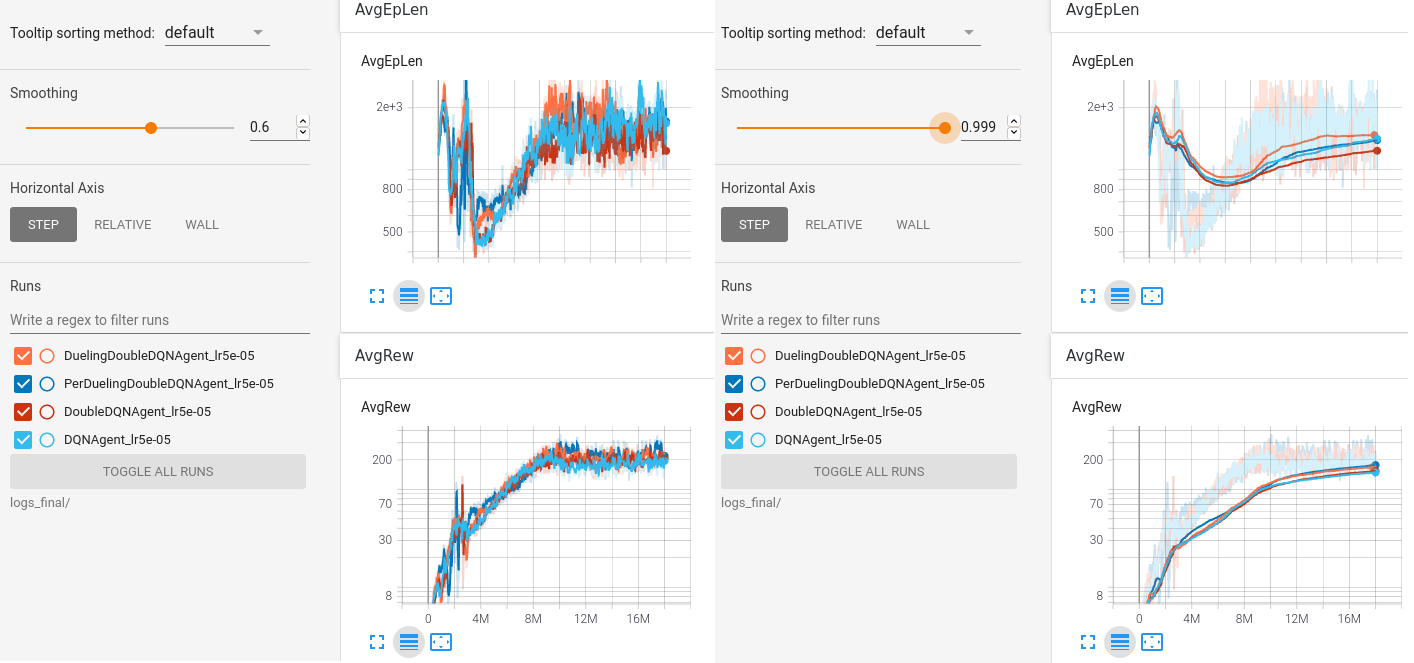
\includegraphics[width=\textwidth]{img/I/Selection_100.png}
\centering
\captionsetup{justification=centering}
\caption{Demo, customized environment 1; (1) visual, (2) learning curves.}
\end{figure}

\pagebreak

\textbf{Customized toy environment 2: Flappy Bird} \\
In the second customized toy environment, the agent controls a game character in a clone of the famous "Flappy Bird" game. The character, represented here by a swimming monkey rather than a flying bird, is in the left side of the screen, with a fixed horizontal position. Pipes covering the full height of the screen are generated at regular intervals at the right end of the screen, and traverse the screen from side to side. The monkey can only swim or sink over the vertical axis and must avoid the pipes by passing through a small gap placed at a random height. When the monkey hits a pipe, the episode is terminated and the environment is reset. The agent observes 3 features; the horizontal distance to the next pipe, the vertical distance to the middle of the gap in the next pipe, and whether it is above or under the middle of this gap on the vertical axis. The agent can choose between 2 actions; swimming to go up and doing nothing to sink down. At each timestep, the agent is punished by the squared distance to the horizontal line passing by the middle of the gap in the next pipe, or is not punished after passing a pipe. The tuned hyper-parameters are $\alpha=\num{1e-3}$ with Adam optimizer and Huber loss, $\gamma=0.9$, $\epsilon_{min}=0.01$, $\epsilon_{dec}=2$M with exponential decay, $N=1$M, $N_{min}=1$M, $\tau=\num{1e-3}$ with soft Polyak update, actions are repeated over $k=5$ frames, $M=32$, and a time limit of $5000$ timesteps is set per episode. The neural network is a MLP with two hidden layers of $16$ neurons each and ELU activations, and the agent was trained over 9M timesteps with the Per3DQN+ algorithm. The agent attains optimal performances, beating the game fully. \\
During deployment, it was consistently stopped by time limit early stopping without hitting a pipe, and was therefore tested without time limit. After eight hours, we stopped the game after the agent had passed more than 15000 pipes without loosing a single time.
It is available at: \textbf{\url{https://github.com/romainducrocq/flappy-seamonkai}}.

\begin{figure}[h]
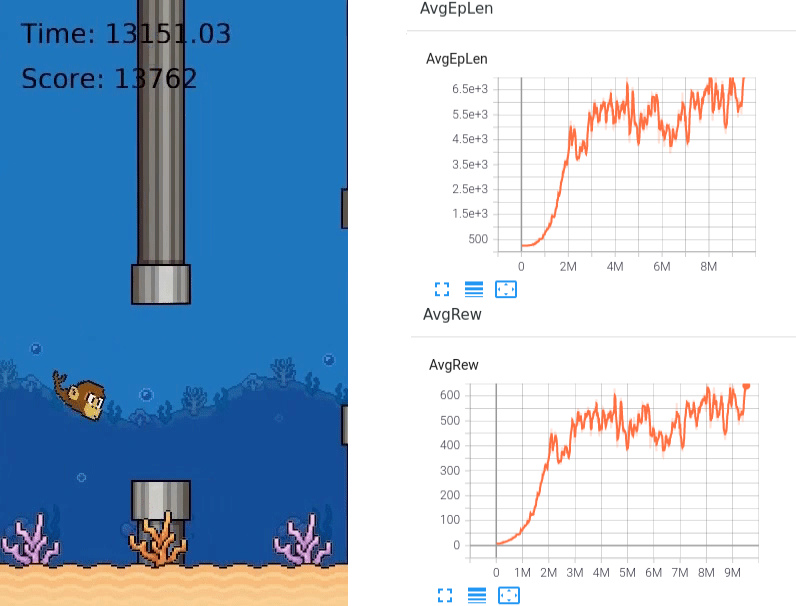
\includegraphics[scale=0.5]{img/I/Selection_101.png}
\centering
\captionsetup{justification=centering}
\caption{Demo, customized environment 2; (1) visual, (2) learning curves.}
\end{figure}

\pagebreak